\documentclass[12pt]{article}

% --- Paquetes comunes ---
\usepackage[utf8]{inputenc}
\usepackage[T1]{fontenc}
\usepackage[spanish]{babel}
\usepackage{amsmath}
\usepackage{amssymb}
\usepackage{hyperref}
\usepackage{graphicx} % <--- ¡NUEVO! Paquete para incluir imágenes
\usepackage{float}

% --- Configuración de márgenes (opcional, para una mejor presentación) ---
\usepackage[margin=2.5cm]{geometry}

% --- Información del documento ---
\title{Práctica 1: Nombre de tu Tarea}
\author{
  Nombre del Estudiante \\
  \texttt{corredsdholaaaao@ejemplo.com}
  \and
  Nombre del Docente \\
  Materia
}
\date{\today}

\begin{document}

% --- Portada ---
\maketitle
\thispagestyle{empty} % No pone el número de página en la portada

\clearpage
\pagenumbering{arabic} % Empieza a numerar las páginas a partir de aquí

\section{Implementación}
\begin{figure}[h!]
    \centering
    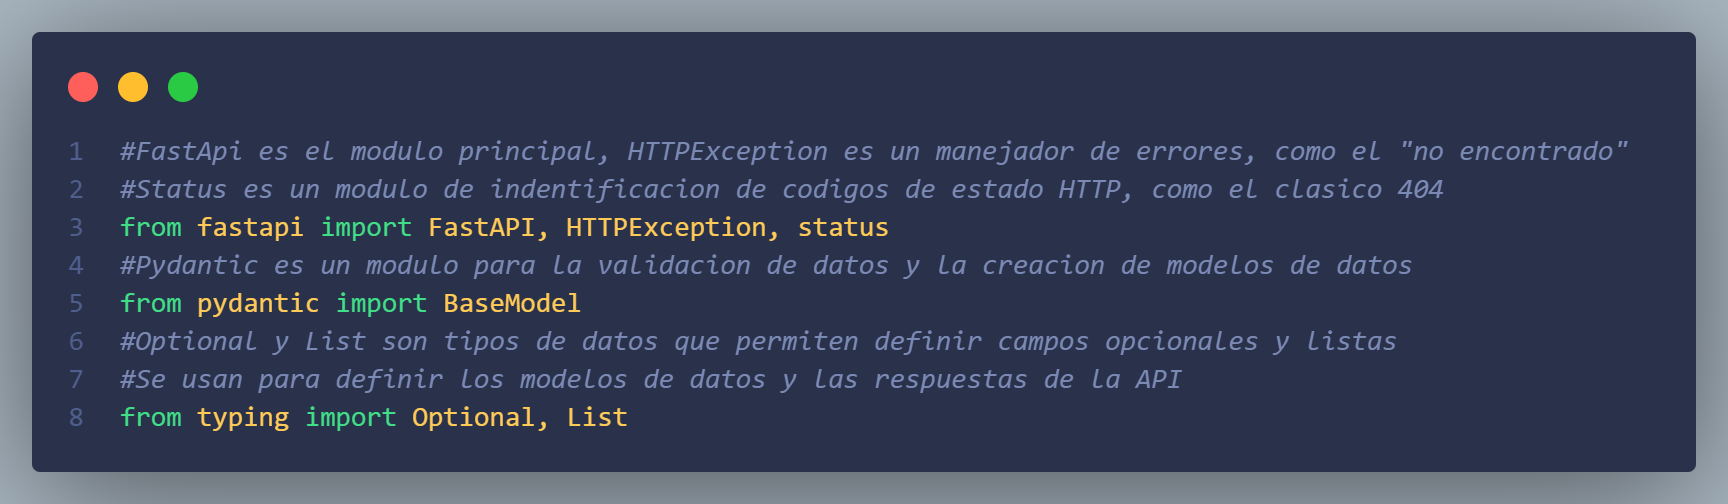
\includegraphics[width=1\textwidth]{Imagenes/Captura1_librerias.png}
\end{figure}

En este apartado se tienen los modulos a utilziar para el funcionamiento de la practica.\\
FastApi nos permite contruir APIS de manera rapida y sencilla, permitiendo definir rutas y manejar solicitudes HTTP de manera eficiente.\\
Las rutas que utilizaremos en esta practica son: GET, POST, PUT y DELETE.\\
Utilizamos Pydantic para validad entradas y para la creacion de un modelo de datos, que en es este caso sera para tener la id de un objeto, y su respectivo contenido.\\
Optional y list son tipos de datos que nos permiten definir atributos que pueden ser opcionales y listas respectivamente.\\


\begin{figure}[h!]
    \centering
    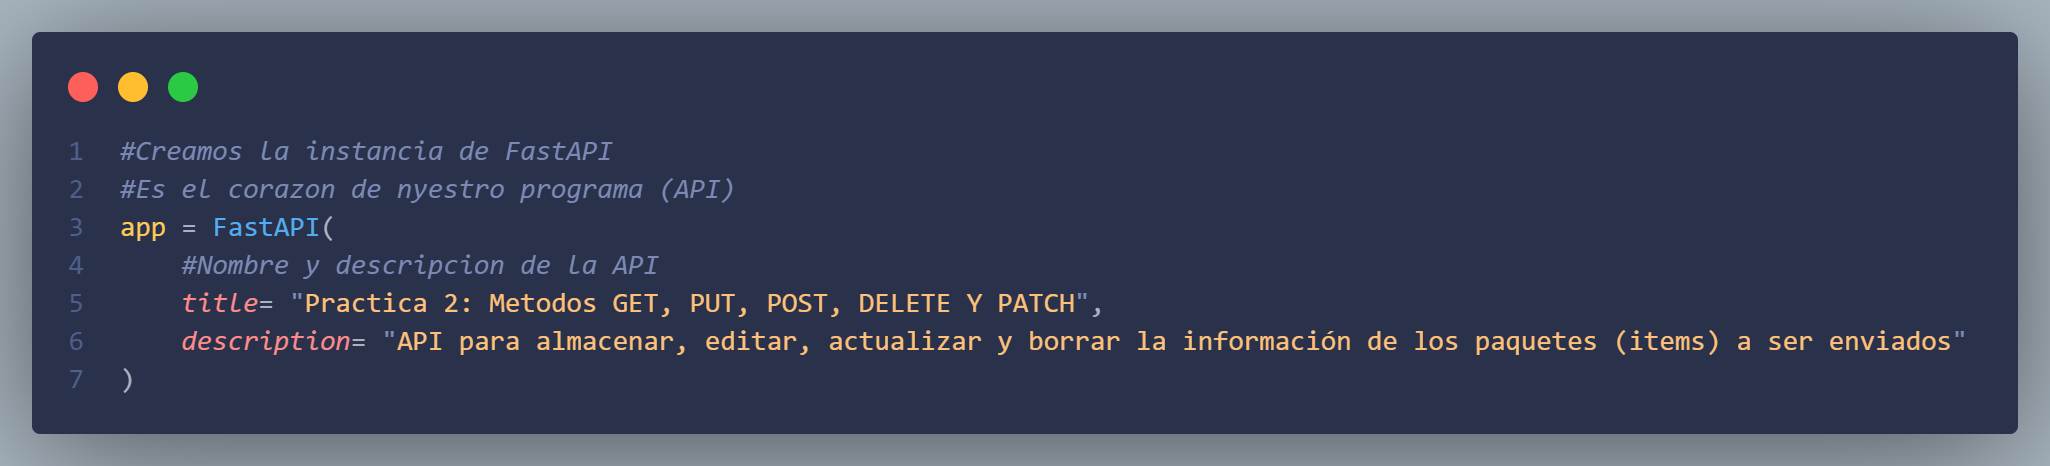
\includegraphics[width=1\textwidth]{Imagenes/Captura2_corazon del programa.png}
\end{figure}

Iniciamos con el corazon de nuestro programa, que es la instancia de FastAPI, en donde definimos el nombre y la descripcion de la API.\\

\begin{figure}[H]
    \centering
    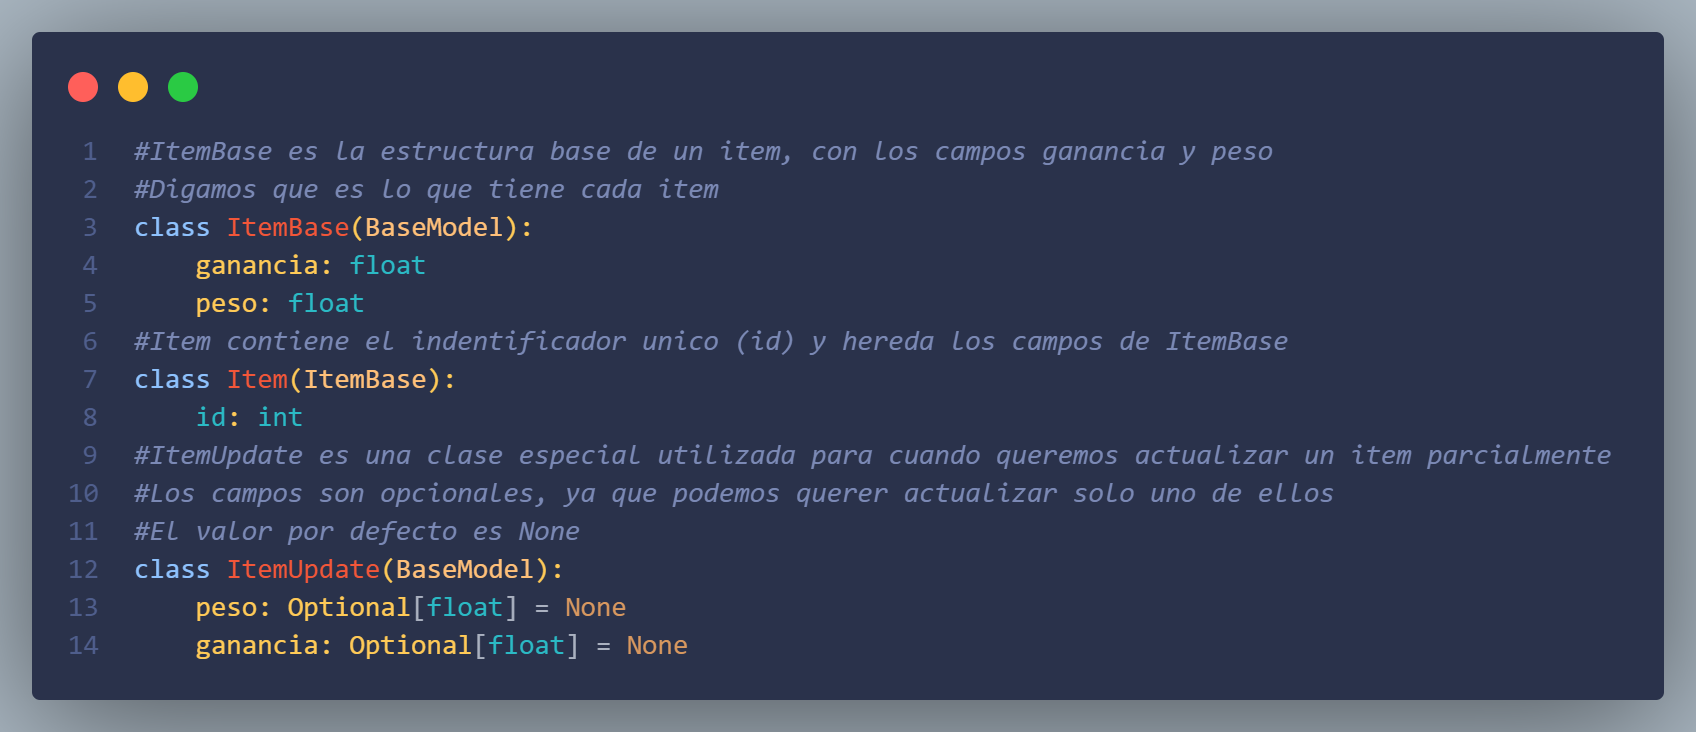
\includegraphics[width=1\textwidth]{Imagenes/Captura3_esctructuradatos.png}
\end{figure}

Gracias a Pydantic, podemos crear una estructura de datos para nuestros objetos a utilizar.
Se tiene un id de tipo entero, este servira para identificar cada objeto.
Cda objeto tiene un contenido de datos, en este caso cuenta con ganancia y perso, ambos de tipo flotante.
Además se tiene una estrcutura para actualizar los datos parcialmente, los campos son opcionales, esto es debido a que no es obligatorio actualizar ambos.

\begin{figure}[H]
    \centering
    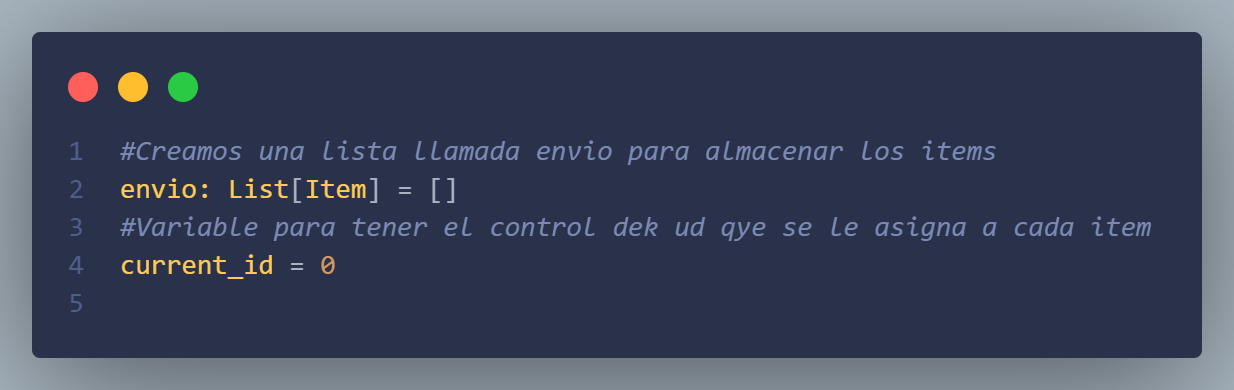
\includegraphics[width=1\textwidth]{Imagenes/Captura4_variablesGlobales.png}
\end{figure}
Utilizamos variables globales para almacenar los objetos y llevar un control del id.
El id se inicializa en 0, y se incrementa cada vez que se crea un nuevo objeto.
Los objetos se almacenan en una lista, que inicialmente esta vacia.
\end{document}